\documentclass{article}
\usepackage{arxiv}

\usepackage[utf8]{inputenc}
\usepackage[english, russian]{babel}
\usepackage[T1]{fontenc}
\usepackage{url}
\usepackage{booktabs}
\usepackage{amsfonts}
\usepackage{nicefrac}
\usepackage{microtype}
\usepackage{lipsum}
\usepackage{graphicx}
\usepackage{natbib}
\usepackage{doi}



\title{Выделение элементов реакции на электроэнцефалограмме}

\author{ Никишкина Евгения Геннадьевна \\
    Кафедра Математических Методов Прогнозирования\\
	Факультет Вычислительной Математики и Кибернетики\\
	Московский государственный университет имени М. В. Ломоносова\\
    Научный руководитель: Майсурадзе Арчил Ивериевич \\
	\texttt{nikishkina.jane@gmail.com} \\
	%% examples of more authors
	} \\
	%% \AND
	%% Coauthor \\
	%% Affiliation \\
	%% Address \\
	%% \texttt{email} \\
	%% \And
	%% Coauthor \\
	%% Affiliation \\
	%% Address \\
	%% \texttt{email} \\
	%% \And
	%% Coauthor \\
	%% Affiliation \\
	%% Address \\
	%% \texttt{email} \\
}
\date{}

\renewcommand{\shorttitle}{\textit{arXiv} Template}

%%% Add PDF metadata to help others organize their library
%%% Once the PDF is generated, you can check the metadata with
%%% $ pdfinfo template.pdf
\hypersetup{
pdftitle={Выделение элементов реакции на электроэнцефалограмме},
pdfsubject={Machine Learning},
pdfauthor={Никишкина Евгения Геннадьевна},
pdfkeywords={First keyword, Second keyword, More},
}

\begin{document}
\maketitle

\begin{abstract}
	Изменения в эмоциональном состоянии человека могут влиять на сигналы электроэнцефалограммы (ЭЭГ). Распознавание и анализ эмоций с использованием биологических сигналов мозга является сложной задачей, требующей точной обработки и выделения признаков для определения наличия эмоции у конкретного человека. Целью данной работы было создание эффективного алгоритма для распознавания эмоций человека на основе анализа рядов ЭЭГ. Были проанализированы различные подходы, в результате чего был выбран оптимальный метод, который затем был реализован в собственной программе. Также были проведены эксперименты на основе подобранных рядов ЭЭГ, содержащих данные об эмоциональных состояниях. Для детектирования эмоций в рядах ЭЭГ был использован новый подход, основанный на анализе аномалий. Результаты экспериментов продемонстрировали, что разработанный алгоритм позволяет получать интерпретируемые результаты по определению наличия эмоций у человека.
\end{abstract}


\keywords{Электроэнцефалография (ЭЭГ) \and Временный ряды \and Детектирование аномалий \and Распознавание эмоций \and SEED dataset \and Глубинное обучение} 

\section{Introduction}
Эмоции представляют собой проявления не только физиологических состояний, связанных с разнообразными чувствами, мыслями и поведением людей, но и психологических откликов на множество внешних стимулов. Умение точно распознавать эмоции играет ключевую роль во множестве сфер. С быстрым развитием науки и техники распознавание эмоций стало широко использоваться в различных областях, таких как взаимодействие человека и компьютера (HCI) \citep{HCI}, здравоохранение \citep{healtcare}, интернет-образование \citep{inted}, мониторинг безопасности \citep{security}, психологический анализ \citep{psych}, а также индустрия развлечений \citep{entern}. Например, распознавание эмоций может оказаться весьма полезным для диагностики таких психических заболеваний, как депрессия и шизофрения \citep{schizophrenia}. Также при взаимодействии человека с компьютером извлеченные эмоции могут использоваться как своего рода обратная связь для предоставления лучшего контента, улучшающего пользовательский опыт в электронном обучении, компьютерных играх и поиске информации.

В последние годы существующие модели распознавания эмоций были разделены на две категории: методы, основанные на физиологических сигналах, и методы, основанные на нефизиологических сигналах. По сравнению с нефизиологическими сигналами, физиологические сигналы не восприимчивы к субъективным факторам, которые могут достоверно отображать эмоциональные состояния человека. Таким образом, распознавание эмоций, основанное на физиологических сигналах, имеет большие преимущества в надежности и практичности \citep{sensors}. В данной статье объектом исследования являются реальные временные ряды, а именно, — записи электроэнцефалограммы. Временной ряд представляет собой собранный в разные моменты времени статистический материал о значении каких-либо параметров исследуемого процесса. Каждая единица статистического материала называется измерением или отсчётом, причем для каждого отсчёта должно быть указано время или порядковый номер измерения. Важно отметить, что при анализе временного ряда учитывается взаимосвязь измерений со временем, что отличает его от простой выборки данных, где учитывается только статистическое разнообразие и характеристики выборки. В области исследований, основанных на физиологических сигналах, ЭЭГ - это спонтанный, несубъективный физиологический сигнал, который может объективно отражать эмоциональные состояния человека \citep{eeg}. В данной работе объектом исследования являются реальные временные ряды, а именно, — записи электроэнцефалограммы. Электроэнцефалография (ЭЭГ) является методом исследования электрической активности мозга путем размещения электродов в определенных зонах на поверхности головы. Данные, полученные таким образом, представляют собой многомерный временной ряд (каждый датчик отвечает за одномерный временной ряд), то есть система из нескольких одномерных рядов, где целевые значения зависят не только от предыдущих значений одного временного ряда, но и от значений дополнительных временных рядов.

Методы распознавания эмоций на основе ЭЭГ можно разделить на две группы: методы классического машинного обучения и глубокого обучения. В методах распознавания эмоций, основанных на классическом машинном обучении, признаки извлекаются вручную для последующего использования в статистических методах, метрических, модельных методов, таких как, например, метод опорных векторов (SVM) \citet{scholkopfsuppor} и Isolation Forest \citet{liu2008isolation}. Лин и др. \citet{sensors18} представили общий процесс традиционных методов машинного обучения для распознавания эмоций по ЭЭГ, включая регистрацию эмоций, получение сигнала, выделение признаков, последующие распознавание или классификация эмоций и т.д. Однако, с такими подходами возникает проблема: из-за нелинейности и высокой размерности сигналов ЭЭГ, методы, эффективные на линейных и низкоразмерных данных, не обеспечивают высокое качество решения сложных задач. Также данные подходы имеет существенный недостаток, заключающийся в том, что процесс извлечения признаков обычно громоздок и в значительной степени зависит от экспертов-людей. Однако трудно получить все подразумеваемые признаки путем извлечения вручную, и используемые формулы часто очень сложны. Кроме того, сигналы ЭЭГ чувствительны к шумам, таким как электромиографические артефакты, которые создают серьезные помехи. Ввиду вышеуказанных трудностей для решения этих проблем используются некоторые методы глубокого обучения. Альхагри и др. \citep{lstm} предложили LSTM для изучения особенностей по сигналам ЭЭГ, затем в качестве классификатора используется полносвязный слой. Для оценки представленного метода использовался набор данных DEAP, который дает среднюю точность $85,65\%$, $85,45\%$ и $87,99\%$ для классов возбуждения, валентности и симпатии соответственно. Предложенный метод обеспечил высокую среднюю точность по сравнению с традиционными методами. Ширрмейстер и др. \citep{cnn} использовали сверточные нейронные сети (CNN) для декодирования и визуализации ЭЭГ, которые продемонстрировали большой потенциал при применении к сквозному распознаванию эмоций на основе ЭЭГ-сигналов, тем самым подтвердив превосходство глубоких нейронных сетей в задачах классификации ЭЭГ. В последние годы CNN (Yea-Hoon et al., 2018; Dm et al., 2021; Keelawat et al., 2021), LSTM (Li et al., 2017; Liu et al., 2017; Sharma et al., 2020), Generative Adversarial Network (GAN) (Luo, 2018) и другие сетевые модели широко использовались при распознавании эмоций по ЭЭГ.

В данной статье используется совершенно новый подход к распознованию эмоций, основанный на детектировании аномалий. Существует множество эффективных методов детектирования аномалий в многомерных временных рядах. Предложенный метод продемонстрировал интерпретируемые результаты при выявлении элементов реакции на датасете SEED.


\section{Headings: first level}
\label{sec:headings}

\lipsum[4] See Section \ref{sec:headings}.

\subsection{Headings: second level}
\lipsum[5]
\begin{equation}
	\xi _{ij}(t)=P(x_{t}=i,x_{t+1}=j|y,v,w;\theta)= {\frac {\alpha _{i}(t)a^{w_t}_{ij}\beta _{j}(t+1)b^{v_{t+1}}_{j}(y_{t+1})}{\sum _{i=1}^{N} \sum _{j=1}^{N} \alpha _{i}(t)a^{w_t}_{ij}\beta _{j}(t+1)b^{v_{t+1}}_{j}(y_{t+1})}}
\end{equation}

\subsubsection{Headings: third level}
\lipsum[6]

\paragraph{Paragraph}
\lipsum[7]



\section{Examples of citations, figures, tables, references}
\label{sec:others}

\subsection{Citations}
Citations use \verb+natbib+. The documentation may be found at
\begin{center}
	\url{http://mirrors.ctan.org/macros/latex/contrib/natbib/natnotes.pdf}
\end{center}

Here is an example usage of the two main commands (\verb+citet+ and \verb+citep+): Some people thought a thing \citep{kour2014real, hadash2018estimate} but other people thought something else \citep{kour2014fast}. Many people have speculated that if we knew exactly why \citet{kour2014fast} thought this\dots

\subsection{Figures}
\lipsum[10]
See Figure \ref{fig:fig1}. Here is how you add footnotes. \footnote{Sample of the first footnote.}
\lipsum[11]

\begin{figure}
	\centering
	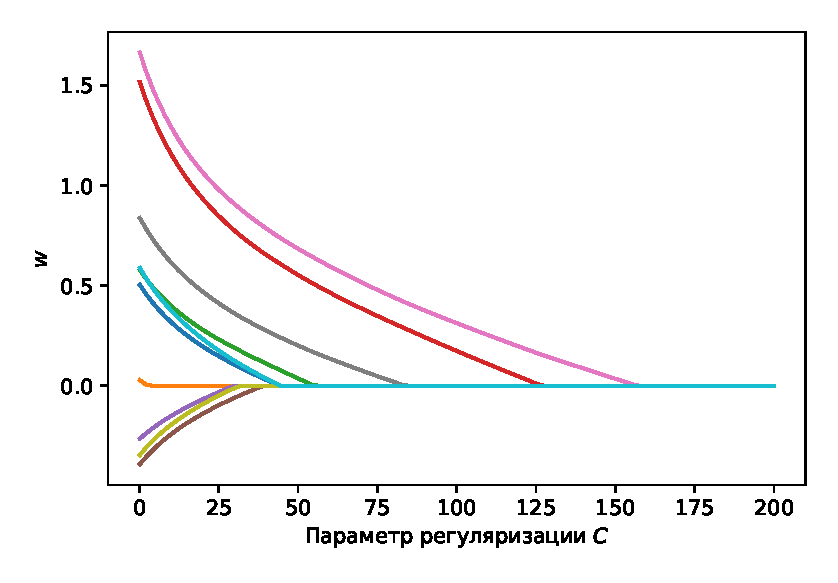
\includegraphics[width=0.5\textwidth]{../figures/log_reg_cs_exp.eps}
	\caption{Sample figure caption.}
	\label{fig:fig1}
\end{figure}

\subsection{Tables}
See awesome Table~\ref{tab:table}.

The documentation for \verb+booktabs+ (`Publication quality tables in LaTeX') is available from:
\begin{center}
	\url{https://www.ctan.org/pkg/booktabs}
\end{center}


\begin{table}
	\caption{Sample table title}
	\centering
	\begin{tabular}{lll}
		\toprule
		\multicolumn{2}{c}{Part}                   \\
		\cmidrule(r){1-2}
		Name     & Description     & Size ($\mu$m) \\
		\midrule
		Dendrite & Input terminal  & $\sim$100     \\
		Axon     & Output terminal & $\sim$10      \\
		Soma     & Cell body       & up to $10^6$  \\
		\bottomrule
	\end{tabular}
	\label{tab:table}
\end{table}

\subsection{Lists}
\begin{itemize}
	\item Lorem ipsum dolor sit amet
	\item consectetur adipiscing elit.
	\item Aliquam dignissim blandit est, in dictum tortor gravida eget. In ac rutrum magna.
\end{itemize}


\bibliographystyle{unsrtnat}
\bibliography{references}

\end{document}
